\documentclass{article}

\usepackage{polski}
\usepackage{amsmath, array}
\usepackage{graphicx}
\usepackage{float}
\usepackage{subfig}
\usepackage{multirow}
\usepackage{enumitem}

\title{Laboratorium 10}
\author{\textbf{Łukasz Wala}\\
    \textit{AGH, Wydział Informatyki, Elektroniki i Telekomunikacji} \\
    \textit{Teoria Współbieżności 2022/23}}
\date{Kraków, \today}

\begin{document}
\maketitle

\section{Zadanie 1}
Rozważmy zbiór zmiennych („bazę danych”) $\{x, y, z\}$
i następujący zbiór akcji („transakcji”) modyfikujących wartości tych zmiennych:

\begin{enumerate}[label=\alph*)]
    \item
    $x := x + y$
    \item
    $y := y + 2z$
    \item
    $x := 3x + z$
    \item
    $z := y - z$.
\end{enumerate}

Akcje możemy wykonywać współbieżnie z następującym zastrzeżeniem: akcja zmieniająca 
wartość zmiennej nie może być wykonana współbieżnie z akcją odczytującą lub modyfikującą 
stan tej samej zmiennej. W języku teorii śladów: dwie akcje są zależne jeśli obie operują 
na tej samej zmiennej, a przynajmniej jedna z nich modyfikuje wartość tej zmiennej.

\subsection{Zadanie 1a}
W alfabecie $A = \{ a, b, c, d\}$ określ relacje zależności i niezależności.

Relacja zależności:
$$ D = \{ (a,a), (a,b), (a,c), (b,a), (b,b), (b,d), (c,a), (c,c), (c,d), (d,b), (d,c), (d,d)\} $$

Relacja niezależności:
$$ I = \{ (a,d), (d,a), (b,c), (c,b)\} $$

\subsection{Zadanie 1b}
Wyznacz ślad wyznaczony przez słowo $w = baadcb$ względem powyższej relacji niezależności.

$$ [baadcb]_I = \{ baadcb, badacb, baadbc, badabc, bdaabc, bdaacb\} $$

Jeżeli sąsiednie operacje są niezależne, można je zamienić kolejnością.

\subsection{Zadanie 1c}
Wyznacz postać normalną Foaty śladu $[w]$.

\begin{table}[h]
\centering
\begin{tabular}{cccc}
\multicolumn{1}{|c|}{}  & \multicolumn{1}{c|}{}  & \multicolumn{1}{c|}{}  & \multicolumn{1}{c|}{}  \\
\multicolumn{1}{|c|}{*} & \multicolumn{1}{c|}{b} & \multicolumn{1}{c|}{}  & \multicolumn{1}{c|}{}  \\
\multicolumn{1}{|c|}{a} & \multicolumn{1}{c|}{*} & \multicolumn{1}{c|}{*} & \multicolumn{1}{c|}{*} \\
\multicolumn{1}{|c|}{a} & \multicolumn{1}{c|}{*} & \multicolumn{1}{c|}{*} & \multicolumn{1}{c|}{d} \\
\multicolumn{1}{|c|}{*} & \multicolumn{1}{c|}{*} & \multicolumn{1}{c|}{*} & \multicolumn{1}{c|}{*} \\
\multicolumn{1}{|c|}{*} & \multicolumn{1}{c|}{b} & \multicolumn{1}{c|}{c} & \multicolumn{1}{c|}{*} \\ \hline
\multicolumn{1}{l}{a}   & \multicolumn{1}{l}{b}  & \multicolumn{1}{l}{c}  & \multicolumn{1}{l}{d} 
\end{tabular}
\end{table}

$$ [w] = (b)(ad)(a)(bc) $$

\subsection{Zadanie 1d}
Narysuj graf zależności Diekerta (w postaci zminimalizowanej - bez krawędzi "przechodnich") dla słowa $w$.

\begin{figure}[H]
    \centering
    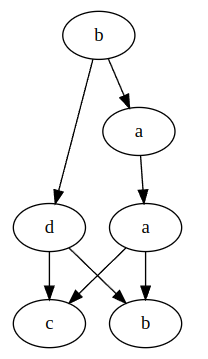
\includegraphics[width=0.4\textwidth]{graph_1.png}
    \caption{graf zależności Diekerta dla słowa $w$}
\end{figure}

\section{Zadanie 2}
Dany jest zbiór akcji:

\begin{enumerate}[label=\alph*)]
    \item
    $x := y + z$
    \item
    $y := x + w + y$
    \item
    $x := x + y + v$
    \item
    $w := v + z$
    \item
    $v := x + v + w$
    \item
    $z := y + z + v$.
\end{enumerate}

\subsection{Zadanie 2a}
W alfabecie $A = \{ a, b, c, d, e, f\}$ określ relacje zależności i niezależności.

Relacja zależności:
\begin{multline*}
D = sym\{ (a,a), (a,b), (a,c), (a,e), (a,f), (b,b), (b,c), (b,d), \\
(b,f), (c,c), (c,e), (d,e), (d,f), (e,e), (e,f), (f,f) \}
\end{multline*}
 
Relacja niezależności:
$$ I = sym\{ (a,d), (b,e), (c,d), (c,f) \} $$

\subsection{Zadanie 2b}
Wyznacz postać normalną Foaty śladu $[u], u = acdcfbbe$.

\begin{table}[h]
\centering
\begin{tabular}{ccccll}
\multicolumn{1}{|l|}{}  & \multicolumn{1}{l|}{}  & \multicolumn{1}{l|}{}  & \multicolumn{1}{l|}{}  & \multicolumn{1}{l|}{}  & \multicolumn{1}{l|}{}  \\
\multicolumn{1}{|l|}{a} & \multicolumn{1}{l|}{*} & \multicolumn{1}{l|}{}  & \multicolumn{1}{l|}{}  & \multicolumn{1}{l|}{}  & \multicolumn{1}{l|}{}  \\
\multicolumn{1}{|c|}{*} & \multicolumn{1}{c|}{*} & \multicolumn{1}{c|}{*} & \multicolumn{1}{c|}{}  & \multicolumn{1}{l|}{*} & \multicolumn{1}{l|}{*} \\
\multicolumn{1}{|c|}{*} & \multicolumn{1}{c|}{*} & \multicolumn{1}{c|}{c} & \multicolumn{1}{c|}{d} & \multicolumn{1}{l|}{*} & \multicolumn{1}{l|}{*} \\
\multicolumn{1}{|c|}{*} & \multicolumn{1}{c|}{*} & \multicolumn{1}{c|}{c} & \multicolumn{1}{c|}{*} & \multicolumn{1}{l|}{*} & \multicolumn{1}{l|}{f} \\
\multicolumn{1}{|c|}{*} & \multicolumn{1}{c|}{*} & \multicolumn{1}{c|}{*} & \multicolumn{1}{c|}{*} & \multicolumn{1}{l|}{*} & \multicolumn{1}{l|}{*} \\
\multicolumn{1}{|c|}{*} & \multicolumn{1}{c|}{b} & \multicolumn{1}{c|}{*} & \multicolumn{1}{c|}{*} & \multicolumn{1}{l|}{*} & \multicolumn{1}{l|}{*} \\
\multicolumn{1}{|c|}{*} & \multicolumn{1}{c|}{b} & \multicolumn{1}{c|}{*} & \multicolumn{1}{c|}{*} & \multicolumn{1}{l|}{e} & \multicolumn{1}{l|}{*} \\ \hline
\multicolumn{1}{l}{a}   & \multicolumn{1}{l}{b}  & \multicolumn{1}{l}{c}  & \multicolumn{1}{l}{d}  & e                      & f                     
\end{tabular}
\end{table}

$$ [u] =  (ad)(cf)(c)(be)(b)$$

\subsection{Zadanie 2c}
Narysuj graf zależności Diekerta (w postaci zminimalizowanej - bez krawędzi "przechodnich") dla słowa $u$.

\begin{figure}[H]
    \centering
    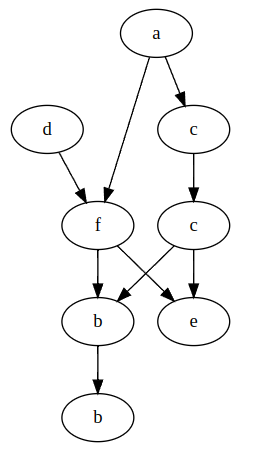
\includegraphics[width=0.4\textwidth]{graph_2.png}
    \caption{graf zależności Diekerta dla słowa $u$}
\end{figure}

\section{Bibliografia}

\begin{enumerate}
    \item
    Volker Diekert, Yves Métivier - Partial Commutation and Traces
\end{enumerate}

\end{document}